
\appendix

\section*{Appendix}

\begin{frame}[label=algorithm]{The algorithm in action.}{Computation of
    the partial order.}
  \begin{columns}[t]
    \column{.4\textwidth}
    \begin{exampleblock}{Genotype matrix}
      $G\colon$
      \begin{tabular}{ccccc}
        A & B & C & D & E \\\hline
        2 & 2 & 2 & 2 & 2 \\
        0 & 1 & 2 & 1 & 0 \\
        1 & 0 & 0 & 1 & 2 \\
        0 & 2 & 2 & 0 & 0
      \end{tabular}
    \end{exampleblock}
    \column{.6\textwidth}
    \begin{exampleblock}{Partial order}
      \begin{tikzpicture}[node distance=15mm]
        \tikzstyle{every node}=
        [%
          fill=green!50!black!20,%
          draw=green!50!black,%
          minimum size=7mm,%
          circle,%
          thick%
        ]

        \node (A) {A};
        \node (B) [right of=A] {B};
        \node (C) [below of=B] {C};
        \node (D) [above of=A] {D};
        \node (E) [below of=A] {E};

        \path [thick,shorten >=1pt,-stealth'] (A) edge (E)
                         (B) edge (C)
                         (D) edge (A)
                             edge[bend right] (E);

        \uncover<2>{
        \path [-,blue,thick](A) edge (B)
                                edge (C)  
                            (B) edge (E)
                            (C) edge (E);}
      \end{tikzpicture}

      Partial order: \tikz[baseline] \draw[thick,-stealth'] (0pt,.5ex)
      -- (5mm,.5ex); 

      \uncover<2>{\textcolor{blue}{Compatible as children of root:
          \tikz[baseline] \draw[thick] (0pt,.5ex) -- (5mm,.5ex);}} 
    \end{exampleblock}
  \end{columns}  
\end{frame}

\begin{frame}{The algorithm in action.}{The matching in the special graph.}
  \begin{columns}[t]
    \column{.3\textwidth}
    \begin{exampleblock}{Partial order}
      \begin{tikzpicture}[node distance=15mm]
        \tikzstyle{every node}=%
        [%
          fill=green!50!black!20,%
          draw=green!50!black,%
          minimum size=8mm,%
          circle,%
          thick%
        ]

        \node (A)              {$A$};
        \node (B) [right of=A] {$B$};
        \node (C) [below of=B] {$C$};
        \node (D) [above of=A] {$D$};
        \node (E) [below of=A] {$E$};

        \path [thick,shorten >=1pt,-stealth'] (A) edge (E)
                         (B) edge (C)
                         (D) edge (A)
                             edge[bend right] (E);

        \path [-,blue,thick](A) edge (B)
                                edge (C)  
                            (B) edge (E)
                            (C) edge (E);

        \only<3->
        {
          \path[very thick,shorten >=1pt,-stealth',red] (D) edge (A) (B) edge (C);
          \path [-,red,very thick](E) edge (B);
        }
      \end{tikzpicture}
    \end{exampleblock}
    \column{.7\textwidth}
    \begin{exampleblock}{Matching graph}
      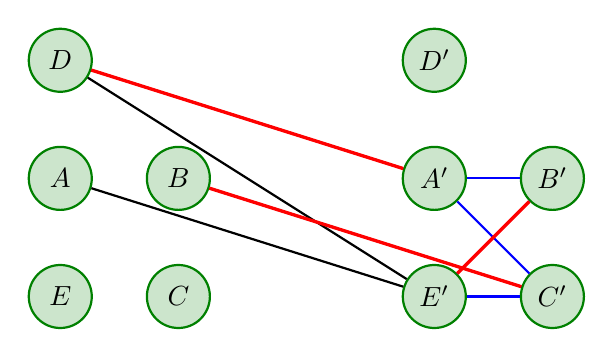
\begin{tikzpicture}[node distance=15mm]
        \tikzstyle{every node}=%
        [%
          fill=green!50!black!20,%
          draw=green!50!black,%
          minimum size=8mm,%
          circle,%
          thick,%
          inner sep=0pt%
        ]

        \node (A)              {$A$};
        \node (B) [right of=A] {$B$};
        \node (C) [below of=B] {$C$};
        \node (D) [above of=A] {$D$};
        \node (E) [below of=A] {$E$};

        \begin{scope}[xshift=4.75cm]
          \node (A')               {$A'$};
          \node (B') [right of=A'] {$B'$};
          \node (C') [below of=B'] {$C'$};
          \node (D') [above of=A'] {$D'$};
          \node (E') [below of=A'] {$E'$};
        \end{scope}
        
        \path [thick]    (A) edge (E')
                         (B) edge (C')
                         (D) edge (A')
                             edge (E');

        \path [blue,thick](A') edge (B')
                               edge (C')  
                          (B') edge (E')
                          (C') edge (E');

        \only<2->
        {
          \path[very thick,red] (D) edge (A')
                           (B) edge (C')
                           (B') edge (E');
        }
      \end{tikzpicture}
    \end{exampleblock}
  \end{columns}

  \medskip
  \uncover<2->{A \alert{maximal matching} in the matching graph
    \uncover<3>{induces\\ \alert{perfect path phylogenies}.}}

  \hfill\hyperlink{return}{\beamerreturnbutton{Return}}
\end{frame}
